\documentclass{beamer}

\beamertemplatenavigationsymbolsempty

\mode<presentation>
{
  \usetheme{default}
}

\usepackage[english]{babel}
\usepackage[latin1]{inputenc}
\usepackage{bussproofs}
\usepackage[retainorgcmds]{IEEEtrantools}

% needs debian package texlive-math-extra
\usepackage{stmaryrd} % for \llbracket, \rrbracket

\usepackage{times}
\usepackage[T1]{fontenc}
% Or whatever. Note that the encoding and the font should match. If T1
% does not look nice, try deleting the line with the fontenc.

\usepackage{tikz}
\usetikzlibrary{positioning}
\usetikzlibrary{calc}
\usetikzlibrary{matrix}
\usetikzlibrary{arrows}


\newcommand{\product}{\!\times\!}
\newcommand{\aand}{\ \wedge \ }
\newcommand{\oor}{\ \vee \ }
\newcommand{\true}{\text{tt}}
\newcommand{\false}{\text{ff}}
\newcommand{\id}{\text{id}}


\title
{Domains for Algebraic Data Types with Computation Steps}

\author
{Markus~Klinik}

\institute[Radboud University Nijmegen]
{
  Radboud University Nijmegen
}

\date
{August 2014}


\newcommand{\arr}{\rightarrow}
\newcommand{\Arr}{\Rightarrow}
\newcommand{\semantics}[1]{\llbracket #1 \rrbracket}
\newcommand{\semanticsFd}[1]{\semantics{#1}_{F\delta}}
\newcommand{\oftype}[2]{#1\!:\!#2}

\begin{document}

\begin{frame}
  \titlepage
\end{frame}

\begin{frame}{Fixpoints, Sums, Products: Pick Two}

\begin{itemize}
\item What? CCC + Fixpoints + Sums = $\lightning$
\item Who? Huwig and Poign\'e, 1990
\item Why? Raising awareness
\item How? Let's see ...
\end{itemize}

\end{frame}


\begin{frame}[fragile]{Preliminaries}

\begin{definition}
A category is \emph{trivial} iff it has one object with one arrow.
\end{definition}

\begin{definition}
A category has \emph{fixpoints} iff every endomorphism has a fixpoint $Yf =
f(Yf)$
\end{definition}

\begin{center}
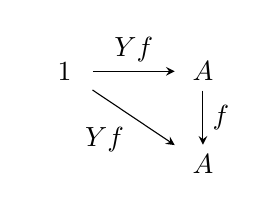
\begin{tikzpicture}
\matrix (m) [matrix of math nodes,row sep=2em,column sep=3em,minimum width=2em
            ,nodes={anchor=center}
            ]
  {
     1 & A \\
     {} & A \\
  };
  \path[-stealth] (m-1-1) edge node [above] {$Yf$} (m-1-2);
  \path[-stealth] (m-1-1) edge node [below left] {$Yf$} (m-2-2);
  \path[-stealth] (m-1-2) edge node [right] {$f$} (m-2-2);
\end{tikzpicture}
\end{center}

\end{frame}



\begin{frame}[fragile]{Warming Up}

\begin{lemma}
In a category with fixpoints, $0 \cong 1$.
\end{lemma}

\vfill

\begin{center}
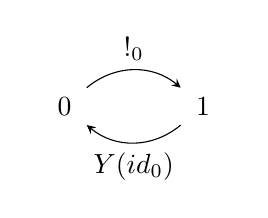
\begin{tikzpicture}
\matrix (m) [matrix of math nodes,row sep=2em,column sep=3em,minimum width=2em]
  {
     0 & 1 \\
  };
  \path[-stealth] (m-1-1) [out=40,in=140] edge node [above] {$!_0$} (m-1-2);
  \path[-stealth] (m-1-2) [out=220, in=320] edge node [below] {$Y(id_0)$} (m-1-1);
\end{tikzpicture}
\end{center}

\end{frame}



\begin{frame}[fragile]{Warming Up}

\begin{lemma}
In a CCC with initial object, for all $A$, $0 \cong 0 \product A$.
\end{lemma}

Existence:
\begin{center}
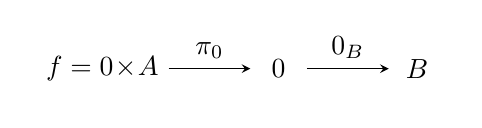
\begin{tikzpicture}
\matrix (m) [matrix of math nodes,row sep=4em,column sep=3em,minimum width=2em
            ,nodes={anchor=center}
            ]
  {
     f = 0 \product A & 0 & B \\
  };
  \path[-stealth] (m-1-1) edge node [above] {$\pi_0$} (m-1-2);
  \path[-stealth] (m-1-2) edge node [above] {$0_B$} (m-1-3);
\end{tikzpicture}
\end{center}

Uniqueness:
\begin{center}
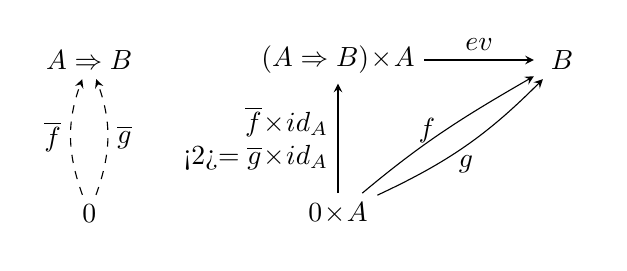
\begin{tikzpicture}
\matrix (m) [matrix of math nodes
            ,row sep=4em
            ,column sep=4em
            ,minimum width=2em
            ,nodes={anchor=center}
            ]
  {
     A \Arr B & (A \Arr B) \product A & B \\
     0 & 0 \product A \\
  };
  \path[-stealth, dashed] (m-2-1) [out=110,in=250] edge node [left] {$\overline{f}$} (m-1-1);
  \onslide<2->{\path[-stealth, dashed] (m-2-1) [out=70,in=290] edge node [right] {$\overline{g}$} (m-1-1);}
  \path[-stealth] (m-1-2) edge node [above] {$\text{ev}$} (m-1-3)
    (m-2-2) edge node [left,align=right] {$\overline{f} \product \id_A$\\{\onslide<2>{$= \overline{g} \product \id_A$}}} (m-1-2)
    (m-2-2) [out=40,in=210] edge node [left] {$f$} (m-1-3);
  \onslide<2->{\path[-stealth] (m-2-2) [out=25,in=225] edge node [below] {$g$} (m-1-3);}
\end{tikzpicture}
\end{center}

\end{frame}


\begin{frame}[fragile]{Warming Up}

\begin{theorem}
Any CCC with fixpoints and initial object is trivial.
\end{theorem}

\begin{equation*}
1\ \cong\ 0\ \cong\ 0 \product A\ \cong\ 1 \product A\ \cong\ A
\end{equation*}

\end{frame}



\begin{frame}[fragile]{But Maybe Binary Sums?}

\begin{theorem}
Any CCC with fixpoints and binary sums is trivial.
\end{theorem}

\begin{lemma}
Any CCC with fixpoints and $1+1$ is trivial.
\end{lemma}

\end{frame}



\begin{frame}[fragile]{Boolean Algebra Objects}
Boolean algebra: $(B,\wedge,\vee,\neg,\true,\false)$ such that
\begin{itemize}
\item $\true = \neg \false$
\item $p = p \aand \true$
\item $\true = p \oor \neg p$
\item ...
\end{itemize}

Boolean algebra object: $(B,\ \wedge, \vee : B\product B \arr B,\ \neg : B \arr B,\ \true, \false : 1 \arr B)$ such that

\begin{center}
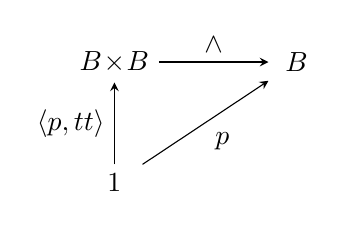
\begin{tikzpicture}
\matrix (m) [matrix of math nodes
            ,row sep=3em
            ,column sep=4em
            ,minimum width=2em
            ,nodes={anchor=center}
            ]
  {
     B \product B & B \\
     1 \\
  };
  \path[-stealth]
    (m-2-1) edge node [left] {$\langle p, \true \rangle$} (m-1-1)
    (m-1-1) edge node [above] {$\wedge$} (m-1-2)
    (m-2-1) edge node [below right] {$p$} (m-1-2) ;
\end{tikzpicture}
\end{center}

\end{frame}



\begin{frame}[fragile]{Why Boolean Algebra Objects?}

\begin{lemma}
The coproduct $1+1$ is a Boolean algebra object.
\end{lemma}

\begin{itemize}
\item $\true, \false$ are the coproduct inclusions $\kappa_0, \kappa_1 : 1 \arr 1+1$
\item $\neg$ is $[\kappa_1, \kappa_0] : 1+1 \arr 1+1$
\item ...
\end{itemize}

\begin{center}
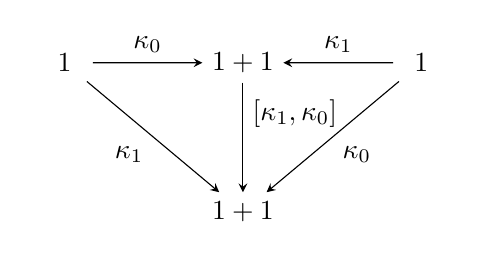
\begin{tikzpicture}[scale=1.2]
\matrix (m) [matrix of math nodes,row sep=4em,column sep=4em,minimum width=2em
            ,nodes={anchor=center}
            ]
  {
     1 & 1 + 1 & 1 \\
     {} & 1 + 1 & {} \\
  };
  \path[-stealth]
    (m-1-1) edge node [below left] {$\kappa_1$} (m-2-2)
            edge node [above] {$\kappa_0$} (m-1-2)
    (m-1-2) edge node [above right] {$[\kappa_1,\kappa_0]$} (m-2-2)
    (m-1-3) edge node [above] {$\kappa_1$} (m-1-2)
            edge node [below right] {$\kappa_0$} (m-2-2)
    ;
\end{tikzpicture}
\end{center}

\end{frame}


\begin{frame}[fragile]{Y Not}
If negation has a fixpoint we are in trouble:\\
Assume $Y \neg = \neg Y \neg$
\begin{IEEEeqnarray*}{rCl}
\true & = & Y\neg \oor \neg Y\neg \\
      & = & Y\neg \oor \phantom{\neg} Y\neg \\
      & = & Y\neg \\
      & = & Y\neg \aand \phantom{\neg} Y\neg \\
      & = & Y\neg \aand \neg Y\neg \\
      & = & \false
\end{IEEEeqnarray*}

In a category with fixpoints and $1+1$, $\neg$ has a fixpoint!\\
Thus $\kappa_0 = \kappa_1 : 1 \arr 1 + 1$
\end{frame}



\begin{frame}[fragile]{Adding Some More Equations}

\begin{itemize}
\item Fact: $- \product A$ preserves coproducts
\item $(1+1)\product A$ is a coproduct of $1 \product A$ and $1 \product A$
\item $(1+1) \product A\ \cong\ A+A$
\item $A+A$ is a coproduct of $A$ and $A$ with $\kappa_0 \product A$ and $\kappa_1 \product A$
\item $\kappa_0 = \kappa_1 \implies \kappa_0 \product A = \kappa_1 \product A$
\end{itemize}


\begin{center}
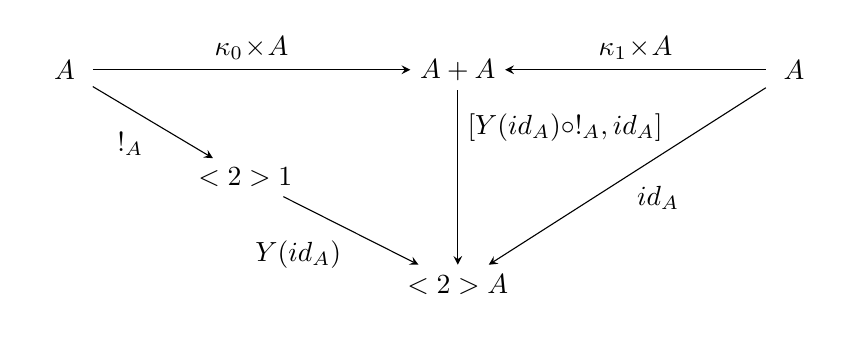
\begin{tikzpicture}
\matrix (m) [matrix of math nodes
            ,row sep=2.5em
            ,column sep=3.5em
            ,minimum width=2em
            ,nodes={anchor=center}
            ]
  {
     A & {} & A + A & {} & A \\
     {} & {\onslide<2>{1}} \\
     {} & {} & {\onslide<2>{A}} \\
  };
  \path[-stealth]
    (m-1-1) edge node [above] {$\kappa_0 \product A$} (m-1-3)
    (m-1-5) edge node [above] {$\kappa_1 \product A$} (m-1-3)
    ;
  \onslide<2>{\path[-stealth]
    (m-1-1) edge node [below left] {$!_A$} (m-2-2)
    (m-1-3) edge node [above=1.8em, right] {$[Y(\id_A) \circ !_A,\id_A]$} (m-3-3)
    (m-1-5) edge node [below right] {$\id_A$} (m-3-3)
    (m-2-2) edge node [below left] {$Y(\id_A)$} (m-3-3)
    ;}
\end{tikzpicture}
\end{center}


\end{frame}


\begin{frame}[fragile]{Conclusion, So Far}

\begin{center}
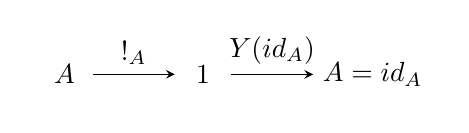
\begin{tikzpicture}
\matrix (m) [matrix of math nodes
            ,row sep=4em
            ,column sep=3em
            ,minimum width=2em
            ,nodes={anchor=center}
            ]
  {
     A & 1 & A = \id_A\\
  };
  \path[-stealth] (m-1-1) edge node [above] {$!_A$} (m-1-2);
  \path[-stealth] (m-1-2) edge node [above] {$Y(\id_A)$} (m-1-3);
\end{tikzpicture}
\end{center}

\begin{center}
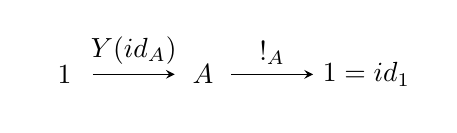
\begin{tikzpicture}
\matrix (m) [matrix of math nodes
            ,row sep=4em
            ,column sep=3em
            ,minimum width=2em
            ,nodes={anchor=center}]
  {
     1 & A & 1 = \id_1\\
  };
  \path[-stealth] (m-1-1) edge node [above] {$Y(\id_A)$} (m-1-2);
  \path[-stealth] (m-1-2) edge node [above] {$!_A$} (m-1-3);
\end{tikzpicture}
\end{center}

In every CCC with fixpoints and $1+1$, for all $A$, $A \cong 1$.

\end{frame}


\end{document}
